%%% Hlavní soubor. Zde se definují základní parametry a odkazuje se na ostatní části. %%%

%% Verze pro jednostranný tisk:
% Okraje: levý 40mm, pravý 25mm, horní a dolní 25mm
% (ale pozor, LaTeX si sám přidává 1in)
\documentclass[12pt,a4paper]{report}
\setlength\textwidth{145mm}
\setlength\textheight{247mm}
\setlength\oddsidemargin{15mm}
\setlength\evensidemargin{15mm}
\setlength\topmargin{0mm}
\setlength\headsep{0mm}
\setlength\headheight{0mm}
% \openright zařídí, aby následující text začínal na pravé straně knihy
\let\openright=\clearpage

%% Pokud tiskneme oboustranně:
% \documentclass[12pt,a4paper,twoside,openright]{report}
% \setlength\textwidth{145mm}
% \setlength\textheight{247mm}
% \setlength\oddsidemargin{15mm}
% \setlength\evensidemargin{0mm}
% \setlength\topmargin{0mm}
% \setlength\headsep{0mm}
% \setlength\headheight{0mm}
% \let\openright=\cleardoublepage

%% Použité kódování znaků: obvykle latin2, cp1250 nebo utf8:
\usepackage[utf8]{inputenc}
%% Ostatní balíčky
\usepackage{graphicx}
\usepackage{amsthm}
\usepackage[outdir=./]{epstopdf}
\usepackage[english]{babel}
\usepackage{blindtext}
\usepackage{booktabs}
\usepackage{caption}
\usepackage{subcaption}
\usepackage{array}
\usepackage{amsmath}
\usepackage{amsfonts}
\usepackage{nccmath}
\usepackage{listings}
\usepackage{alltt}
\usepackage{upquote}

\usepackage{pgfplots}
\usepackage{pgfplotstable}
\usepackage{tikz} % LATEX

\usetikzlibrary{arrows,snakes,backgrounds,automata,backgrounds,calendar,er,folding,matrix,trees,topaths,shapes}

\pgfplotsset{compat=newest}

\usepackage[printonlyused,withpage]{acronym}

%% Balíček hyperref, kterým jdou vyrábět klikací odkazy v PDF,
%% ale hlavně ho používáme k uložení metadat do PDF (včetně obsahu).
%% POZOR, nezapomeňte vyplnit jméno práce a autora.
\usepackage[unicode]{hyperref}   % Musí být za všemi ostatními balíčky
\hypersetup{pdftitle=Development of an English public transport information dialogue system}
\hypersetup{pdfauthor=Martin Vejman}


% \todo{} command.
\usepackage{color}
\newcommand{\todo}[1]{}
\renewcommand{\todo}[1]{{\color{red} TODO: {#1}}}

\newcommand{\ask}[1]{}
\renewcommand{\ask}[1]{{\color{blue} ASK: {#1}}}

%%% Drobné úpravy stylu

% Tato makra přesvědčují mírně ošklivým trikem LaTeX, aby hlavičky kapitol
% sázel příčetněji a nevynechával nad nimi spoustu místa. Směle ignorujte.
\makeatletter
\def\@makechapterhead#1{
  {\parindent \z@ \raggedright \normalfont
   \Huge\bfseries \thechapter. #1
   \par\nobreak
   \vskip 20\p@
}}
\def\@makeschapterhead#1{
  {\parindent \z@ \raggedright \normalfont
   \Huge\bfseries #1
   \par\nobreak
   \vskip 20\p@
}}
\makeatother

% Toto makro definuje kapitolu, která není očíslovaná, ale je uvedena v obsahu.
\def\chapwithtoc#1{
\chapter*{#1}
\addcontentsline{toc}{chapter}{#1}
}

\begin{document}

% Trochu volnější nastavení dělení slov, než je default.
\lefthyphenmin=2
\righthyphenmin=2

%%% Titulní strana práce

\pagestyle{empty}
\begin{center}

\large

Charles University in Prague

\medskip

Faculty of Mathematics and Physics

\vfill

{\bf\Large MASTER THESIS}

\vfill

\centerline{\mbox{\includegraphics[width=60mm]{../img/logo.eps}}}

\vfill
\vspace{5mm}

{\LARGE Martin Vejman}

\vspace{15mm}

% Název práce přesně podle zadání
{\LARGE\bfseries Development of an English public transport information dialogue system}

\vfill

% Název katedry nebo ústavu, kde byla práce oficiálně zadána
% (dle Organizační struktury MFF UK)
Institute of Formal and Applied Linguistics

\vfill

\begin{tabular}{rl}

Supervisor of the master thesis: & Mgr. Ing. Filip Jurčíček Ph.D. \\
\noalign{\vspace{2mm}}
Study programme: & Informatics \\
\noalign{\vspace{2mm}}
Specialization: & Theoretical Computer Science \\
\end{tabular}

\vfill

% Zde doplňte rok
Prague 2015

\end{center}

\newpage

%%% Následuje vevázaný list -- kopie podepsaného "Zadání diplomové práce".
%%% Toto zadání NENÍ součástí elektronické verze práce, nescanovat.

%%% Na tomto místě mohou být napsána případná poděkování (vedoucímu práce,
%%% konzultantovi, tomu, kdo zapůjčil software, literaturu apod.)

\openright

\noindent
I thank my supervisor Mgr. Ing. Filip Jurčíček, Ph.D. for his patience and kind critical comments that directed my effort while working on this thesis. \\
I also thank my mother for her continuous support.


\newpage

%%% Strana s čestným prohlášením k diplomové práci

\vglue 0pt plus 1fill


\noindent
I declare that I carried out this master thesis independently, and only with the cited
sources, literature and other professional sources.

\medskip\noindent
I understand that my work relates to the rights and obligations under the Act No.
121/2000 Coll., the Copyright Act, as amended, in particular the fact that the Charles
University in Prague has the right to conclude a license agreement on the use of this
work as a school work pursuant to Section 60 paragraph 1 of the Copyright Act.

\vspace{10mm}

\hbox{\hbox to 0.5\hsize{%
In ........ date ............
\hss}\hbox to 0.5\hsize{%
signature of the author
\hss}}

\vspace{20mm}
\newpage

%%% Povinná informační strana diplomové práce

\vbox to 0.5\vsize{
\setlength\parindent{0mm}
\setlength\parskip{5mm}

Název práce:
Development of an English public transport information dialogue system
% přesně dle zadání

Autor:
Martin Vejman

Katedra:  % Případně Ústav:
Ústav formální a aplikované lingvistiky
% dle Organizační struktury MFF UK

Vedoucí diplomové práce:
Mgr. Ing. Filip Jurčíček, Ph.D.
% dle Organizační struktury MFF UK, případně plný název pracoviště mimo MFF UK

Abstrakt:
% abstrakt v rozsahu 80-200 slov; nejedná se však o opis zadání diplomové práce

Tato práce se zabývá vývojem anglického dialogového systému, který je založen na frameworku Alex určeného pro vytváření dialogových systémů.
Práce popisuje adaptaci komponent frameworku na novou doménu a anglický jazyk.
Výsledný dialogový systém poskytuje informace o veřejné dopravě ve městě New York.
Součástí práce je příprava statistického modelu a nasazení vlastního rozpoznávače řeči pomocí nástrojů Kaldi.
Ve srovnání s Google Speech API s ním bylo dosaženo lepších výsledků, které vychází ze subjektivního hodnocení uživatelů získaného pomocí crowdsourcingu.

% Tato práce se zabývá vývojem anglického dialogového systému, který je založen na frameworku Alex určeného pro vytváření dialogových systémů.
% Systém poskytuje informace o veřejné dopravě ve městě New York.
% Práce popisuje adaptaci komponent frameworku na novou doménu a anglický jazyk.
% %Angličtina rozšiřuje možnosti použití a hlavním přínosem řešení bude sběr dat pro vytváření lepších rozpoznávačů řeči.
% Součástí práce je příprava statistického modelu a nasazení vlastního rozpoznávače řeči pomocí nástrojů Kaldi.
% Ve srovnání s Google Speech API s ním bylo dosaženo lepších výsledků, které vychází ze subjektivního hodnocení uživatelů získaného pomocí crowdsourcingu.

% Angličtina rozšiřuje možnosti použití.
% Hlavním přinosem řešení je 


% Práce popisuje adaptaci komponent frameworku pro novou doménu v 

% Existoval ASDFramework s jednim prototypickych dialogem pro cestinu.
% Ty jsi overil ze lze adaptovat vsechny komponenty ASDF na novou domenu a jazyk (predtim jsme to jen tvrdili),
% a hlavne jsi v praci popsal jak se to dela! (To asi zadny jiny opensource framework nema popsane, ale vsichni tvrdi, ze to umi!)

%Tato práce se zabývá vývojem dialogového systému v angličtině, který je založený na systému Alex vyvíjeném na Ústavu formální a aplikované lingvistiky.
%Řešení zahrnuje implementaci komponent pro porozumění řeči, řízení dialogu a generování odpovědí.
%Součástí práce je otestování systému na reálných uživatelích ze Spojených států pomocí platformy CrowdFlower.
%Pomocí přepisů hovorů byl vytvořen jazykový model pro Kaldi dekodér, který zlepšil schopnost rozpoznání řeči ve srovnání s cloudovým rozpoznávačem od Googlu.
%V minulosti byl vytvořen český systém, který má však omezené možnosti použití.
%Angličtina však rozšiřuje možnosti použití.
%Hlavním přínosem řešení bude sběr dat pro vytváření lepších rozpoznávačů řeči.
%Cílem této práce je vytvořit anglický dialogový systém v angličtině.


% Tato práce se zabývá vývojem dialogového systému v angličtině, který je založený na českém systému Alex.
% Systém poskytuje informace o veřejné dopravě ve městě New York.
% Řešení bylo otestováno na reálných uživatelech pomocí platformy na crowdsoursing.
% Součástí řešení je příprava statistických modelů a nasazení vlastního rozpoznávače řeči pomocí nástrojů Kaldi.
% Ve srovnání s Google Speech API s ním bylo dosaženo lepších výsledků, které vychází ze subjektivního hodnocení uživatelů.


% Vzal jsem hotovy dialogovy system a uspesne ho transformoval pro jiny jazyk a domenu (Tohle me tam chybi opravdu hodne).
% Narazil jsem na problemy takove a takove a v praci popisuji reseni pomoci tohoto a tohoto


Klíčová slova:
strojové učení, automatické rozpoznávání řeči, dialogový systém
%machine learning, automatic speech recognition, spoken dialogue systems
%dialogový systém, crowdsourcing, veřejná doprava, alex
% 3 až 5 klíčových slov

\vss}\nobreak\vbox to 0.49\vsize{
\setlength\parindent{0mm}
\setlength\parskip{5mm}

Title:
Development of an English public transport information dialogue system
% přesný překlad názvu práce v angličtině

Author:
Martin Vejman %Jméno a příjmení autora

Department:
Institute of Formal and Applied Linguistics
% dle Organizační struktury MFF UK v angličtině

Supervisor:
Mgr. Ing. Filip Jurčíček, Ph.D.
% dle Organizační struktury MFF UK, případně plný název pracoviště
% mimo MFF UK v angličtině

Abstract:
This paper presents a development of an English spoken dialogue system based on the Alex dialogue system framework.
The system provides public transport information in New York.
English allows to construct more applicable system.
The main benefit of the solution is the collection of speech data for creating better speech recognizers.
This work involves creating statistical model and deployment of custom Kaldi speech recognizer.
Its performance was notably better in comparison with the Google Speech API.
The comparison was based on a subjective user satisfaction acquired by crowdsourcing. %conducted

% The solution involves the development of spoken language understanding, dialogue manager and language generation components.
% Crowdsourcing platform CrowdFlower is used for collecting speech data and audio transcriptions.
% Collected data are furnished for training a language model and building a Kaldi decoder.
% CrowdFlower is further used for comparison of Google Speech API and Kaldi ASR.
% It is shown that Kaldi recognizer achieves better results in restricted public transport domain.



% abstrakt v rozsahu 80-200 slov v angličtině; nejedná se však o překlad
% zadání diplomové práce

Keywords:
machine learning, automatic speech recognition, spoken dialogue systems
%spoken dialogue system, crowdsourcing, public transport information, Alex% 3 až 5 klíčových slov v angličtině

\vss}

\newpage

%%% Strana s automaticky generovaným obsahem diplomové práce. U matematických
%%% prací je přípustné, aby seznam tabulek a zkratek, existují-li, byl umístěn
%%% na začátku práce, místo na jejím konci.

\openright
\pagestyle{plain}
\setcounter{page}{1}
\tableofcontents

%%% Jednotlivé kapitoly práce jsou pro přehlednost uloženy v samostatných souborech


\chapter*{Introduction}
\addcontentsline{toc}{chapter}{Introduction}

Providing information to consumers is a common task usually solved by implementing a web page or a mobile application.
Spoken dialogue systems on the other hand, are suitable for fulfilling such task while simplifying the access to the information.
Spoken dialogue systems allow people to interact with a computer the most natural way, by voice.
They are intuitive, direct and hands-free, which renders an opportunity for deployment in many fields.
There is no need to find a mobile device and enter queries into some puzzling interface, it is enough to simply say the words.
Despite this, it may serve as a valuable asset for obtaining information for the elderly and especially for blind people and people with visual impairment.%it addresses larger spectrum of people, convenient source of information

However, it is very difficult to implement a dialogue system from ground up.
Fortunately The Alex dialogue system platform\cite{asdf} (ASDF) incorporates all of the key components needed for performing the task.
We decided to take the advantage of ASDF and implement a spoken dialogue system in English for providing public transport information (PTI) in New York.
New York, the city with the highest ridership in the United States and with one of the most extensive subway systems in the world, presents a formidable challenge.
The English language benefits from wider range of use and larger competition to be compared with.
This enables us to build better systems with greater potential.

Automatic speech recognition (ASR) is not yet at the point where the meaning of every utterance could be reliably identified by a computer.\cite{asr}
Although with a restricted domain, it is possible to achieve substantially better results utilizing a trained speech recognizer.
A crowdsourcing platform CrowdFlower will be used to evaluate our PTI solution and to collect speech data.
The collected speech data will be facilitated to train a Kaldi speech recognizer and it will be compared with the Google ASR.
The comparison measures will be based on the Crowdflower contributor's report. % deliberation testimony

Our PTI solution will be a useful showcase of the ASDF and will further contribute to collect speech data for improving the quality of speech recognizers. \ask{should we mention MTA here?} %It will be competing in a MTA app quest competition.

The outcomes of this thesis include the public transport information telephone-based dialogue system for New York, \todo{and the other stuff}.

The paper is organized as follows.
In the first chapter we will look over the used technologies.
In the second chapter we will discuss the implementation in its principles by each component. %at a time
The third chapter will cover the features of implemented solution and display its capabilities.
The fourth chapter will describe the workflows associated with creating such dialogue system.
Training Language model and building Kaldi decoder will also be covered by this chapter.
In the fifth chapter we will draw conclusions and summarize the findings encountered in the process.




% telephone-based spoken dialog system

% The development of dialogue systems makes possible more natural human-computer interaction.
% The dialogue systems have prospects to be increasingly utilized at robotics and for providing information.
% Spoken dialogue systems are being used more frequently for their potential in numerous applications at many different fields.
% Spoken dialogue systems allow a user to interact with a computer using voice as the primary communication medium.

% They are being used for loan establishment, car rental, call rate adjustment etc.
% They may serve for the purposes of renting a car, establishing loans, or changing telephone rates, rezervace hotelu.


% Besides, there is a reason why in every other sci-fi movie, characters communicate with computers solely via voice. It is easy (simple?).



% -----------
% intro
% what's it about
% how to do the experiments
% dokumentace

% showcase systému, english - bigger potential -> better system
% dialog - všichni to dělaj na webovkách, telefonech, některý lidi to ani 

% nemůžou použít(slepý), proto je lepší dialog. 
% motivace - starý, slepí, pohodlnost, nechci vytahovat nic, jen se zeptám

% kapitola-proces, kdybych to dělal pro další doménu, tak co bych udělal 

% 1.2.3....
% tu finální, a potom v diskuzi - zkoušeli jsme to i takhle, ale 
% nefungovalo to pro to a tak.,

% process třeba jenom co obnáší natrénování modelu

% dialog-výhody, omezení
% obecně ds, alex,1:41 PM 4/10/2015 co všechno se musí adaptovat, jak se to musí udělat, co 
% jsem musel změnit u jednotlivých

% evaluace (cf), transkripce
% soutěž
% ----------




%Scientific paper consists of:

%	Introduction
%	Materials and Methods
%	Results
%	Discussion
%(co je známo, cíl práce, je to důležité, volba metody)
%at the end - a paragraph with a structure of the document
%THE INTRODUCTION HAS TO REFLECT THE PROCESS OF THE PAPER. WHAT EXACTLY WILL HE GET LATER SERVED AT THE TEXT.

%INTRODUCTION:

% What is a dialogue system
% Introduction to the problematics
% It is important
% method selection
% what has been done
% what has not been done
% what do we want to display in our work
% apt definition of the goals of this work

%This work is concerned with this and that, the assumptions are these, we would also want to use crowd sourcing for leaning something which enables this and that, then we evaluate


% What is interesting on this thesis: 
%  - It utilizes voice interface for obtaining information.
% Who could utilize output of this thesis:
%  - MTA for sure
% What output could be marked as surprising:
%  - we was able to achieve a comparable results with google TTS.
% What am i most proud of?
%  - The fact that we were able to participate in an MTA contest with a good competitive solution.
% If someone should continue my work - what parts should have he used and what should have he rewritten.
%  - He should use the whole solution, bus he would have to rewrite a SLU and HDC a bit for better handling of the streets and stuff
% What have I learned during the process, who could be interested:
%  - For sure the companies that make similar applications for different domains could be interested.
%  - The ones that want to use ADSF for development of their own dialogue system
%  - I have learned a great deal about dialogue systems, working with crowd sourcing etc.

\chapter{Technologies used}

\section{Alex framework - PTICS}

The Alex Dialogue System Framework (ADSF) is used for utilizing research in the development of spoken dialogue systems.
ADSF is maintained by the dialogue systems group at UFAL \cite{ufal}, the Institute of Formal and Applied Linguistics, Faculty of Mathematics and Physics, Charles University in Prague.
This framework is in Python.

The ADSF consists of baseline components for assembling spoken dialogue systems.
There are tools for processing logs and evaluating spoken dialogue systems.
These tools can be used for audio transcriptions for example.
A small set of example implementations for different domains is also present.

%We will introduce individual components in detail later in this section.
\todo{There may be another paragraph about PTICS ?}

\subsection{Automatic Speech Recognition}

Automatic Speech Recognition (ASR) transforms spoken words into text.
Many applications already use ASR technology as an interface between computer and person, although it is not yet capable of understanding all speech in any environment.
Many factors influence perception of voice. Acoustic conditions, voice differences, distance from recording device, heavy accents even voice emphasis, these are few of the issues versatile ASR has to cope with.
Achieving better quality requires great many hours of transcribed text, which is hard to come by.
However, when we restrict ourselves to a specific domain, the scope of words becomes quite limited.
There is only so many expressions that can be used in a common conversation about particular subject.
Therefore better results can be achieved.

\todo{HMM(AM)->ASR<-N-grams(LM)}

\subsubsection{Kaldi}

Kaldi is an open-source \footnote{Apache License 2.0} toolkit for speech recognition based on finite state transducers commonly used among researchers.
We use python wrapper Pykaldi within the ADSF.

\todo{Process of training and testing Kaldi models will be explained in chapter [whoKnows].}

\subsubsection{Google}

Google has its own cloud solution of ASR which is used by Google command and Google Translate.

\todo{describe it a little bit - take inspiration from code}

\subsubsection{CloudASR}

\todo{Should I even say anything about this?}

\subsubsection{Voice Activity Detection}

In order to send a voice track to ASR processing, we need to be able to cut speech into logical units (sentences).
This role is performed by the Voice Activity Detection (VAD).

\subsection{Text To Speech}

Small but nonetheless crucial part of Dialogue System.
Makes an instantaneous impression as this is the first and in most cases the only output an end user is able to perceive. % comprehend
There are also variety of TTS providers. ADSF supports Flite, VoiceRSS and Google.

\subsection{Dialogue Manager}

\todo{it has to keep inner states for knowing the context, it is the soul of dialogue system}

\subsection{Natural Language Generation}


\subsection{VoIP interface}

\todo{SIP}



\todo{odstavec a obrázek o tom, jak se typicky daj použít dohromady - na příkladu ptics - nebo něco lehčího?}



\section{Crowdsourcing}

Crowdsourcing is a method for acquiring data by delegating work to a community of people.
In particular online communities tend to be employed for convenience.
By dividing tasks into smaller independent parts, one can eliminate the need for expert workers and therefore reduce costs associated with acquisition of the coveted data.
In some cases the cost savings can be a tenfold of what in-house solution may provide \cite{Quality Management on Amazon Mechanical Turk} % offer
However, this method can hardly achieve the quality or accuracy of expert workers. 

There are several crowdsourcing platforms connecting workers with work requesters such as Amazon Mechanical Turk \footnote{\url{https://www.mturk.com/mturk/welcome}}, Samasource \footnote{\url{http://samasource.org/}}, CrowdFlower and many more.
Samasource is a non-profit organization with a noble cause of lifting people out of poverty through digital work.
It does not, however, meet our need of employing native English speakers.
While Amazon Mechanical Turk would meet our requirements, it is no longer available for non-US requesters.
With Crowdflower, we are able to implement a custom solution directly within the platform.

Crowdflower has mechanisms such as monitoring answer distributions and computing confidence score for maintaining quality of the output data. % that yield good quality assurance. the assurance of quality
They claim great amount of contributor force which promises prompt job resolution. % wide range 
The platform contains comprehensible templates for common tasks.
It features interface for building a custom job from scratch with a sensible support and demonstrative examples, too % in form of examples, too.

\chapter{Implementation -- Public Transport Information in New York}

In this chapter we will go through each component that needed to be implemented or modified in \ac{PTINY}.
This excludes automatic speech recognition, text to speech and VoIP interface.
%These components are ready to use.
The principle will be described along with relevant instruments. %apparatus. 
All of these components are domain specific versions of domain independent components of the \ac{ASDF}.

First we will cover keyword database and matching words against the input, than we will describe changing states in our dialogue system.
Last we will explain how the state is translated to the output which will conclude in an outline of utterance processing. % summary of utterance processing.

\section{Spoken Language Understanding}

To be able to process, evaluate and respond to user's requests, semantic meaning needs to be extracted from utterances. %\ac{ASR} hypothesis
This is realized via \acf{SLU}, which uses a vast static keyword database for analyzing words and phrases of each utterance.
Being able to handle such semantic representation makes it possible to change state of the dialogue system.
There are different approaches for \ac{SLU} development.
There are \ac{SLU} techniques based on statistical models learned from data.
We, however, have implemented a handcrafted \ac{SLU} based on simple keyword rules.
Both approaches are supported by the \ac{ASDF} as demonstrated in \cite{slu}.

% \todo{which gives us direct control over the translation process.} % clear overview of the process

\subsubsection{Keyword database} 
% \todo{is this knowledge-base?}

Public transport information domain demands the ability to respond to two major constraint queries - location and time.
The time and supplementary keywords can be defined explicitly or they can be generated by a simple script.
However, the location data are specific for the region we decided to cover and therefore must be gathered.

We ultimately need just the name of the waypoint for the keyword matching process.
However, the stop or city names might be ambiguous which is why we need to keep further knowledge about geographic information and more general area. %realm territory locality region

%For a prompt keyword matching, there is an object kept in memory containing all of the location keywords as well as other PTI related keywords. class label database
\subsubsection{Location data terminals} \label{sec:terminals}

The types of waypoints are streets, stops, boroughs, cities and states.
All of these location categories are listed in a separate file for the convenience of adding new or updating existing entries.
It is obvious that the borough list will be very narrow and may be unnecessary because there is only five boroughs in New York.
But the idea is to be able to distinguish between streets and stops with the same name that are very likely to appear within the same city.
If we decided to expand the system to cover Los Angeles region for example, we might need to add not only LA boroughs but to define a finer administrative division altogether.

In terms of the stops, we collected the latest data from
MTA\footnote{Metropolitan Transportation Authority - \url{http://www.mta.info/}},
PATH\footnote{Port Authority Trans Hudson - \url{http://www.panynj.gov/}},
NJ Transit\footnote{New Jersey Transit - \url{http://www.njtransit.com/}},
NY Waterway\footnote{New York Waterway - \url{http://www.nywaterway.com/}} and
Amtrak\footnote{The National Railroad Passenger Corporation - \url{http://www.amtrak.com/home}} for long-distance trips.
Most of the companies are providing their schedules for developers in a unified format.
The \acf{GTFS} defines a common format for public transportation schedules and associated geographic information.\footnote{GTFS - \url{https://developers.google.com/transit/gtfs/}}

We could adopt the \ac{GTFS} format which would be very convenient for updating \cite{gtfs}.
However, some of the datasets were not strictly following the \ac{GTFS} making it unfeasible to work with.
Missing values, overflowing columns or disunited expressions occurred infrequently, nevertheless throughout notable portion of the data.
The benefit of an easy update and access to additional information did not outweigh the shortcomings encountered.

We opted for a simple format that takes only the most important features into account.
Selecting fewer columns makes it easier to add places that are not available in the \ac{GTFS}.
This includes a few smaller transport companies commuting between tens of terminals that we also included into our database.

In addition to official stops, we added over a hundred of the most popular sites in New York from various top \textit{n} lists.
Those can be used as good reference points in everyday commutes so that the following sentence can be handled for instance.

\begin{flushleft}
\textit{``From Empire State Building to Central Park.''}.
\end{flushleft}

\noindent We used Google Geolocation \ac{API}\footnote{\url{https://developers.google.com/maps/documentation/business/geolocation/}}, to obtain longitude, latitude and borough for each popular site. Geo coordinate information is used when looking for a connection.

The obtained data in raw form can not be used for keyword matching. As opposed to the Czech language, there is no necessity to take inflection into account, however, there is a number of ways to express stop or a street.
Stops in particular, mostly called after an intersections, can be unfolded and expressed in different order and coupled with a different conjunction.

For example the stop \texttt{1 Av/E 111 St} can be expressed as
\begin{flushleft}
\textit{``east hundred eleventh street first avenue''}. \\
\textit{``east hundred eleventh street at first avenue''}. \\
\textit{``east hundred eleventh street and first avenue''}. \\
\hspace{8em} $\vdots$ \\
\textit{``east one hundred and eleventh street at first avenue''}. \\
\hspace{8em} $\vdots$ \\
\textit{``first avenue and east hundred and eleventh street''} \\
\hspace{8em} $\vdots$
\end{flushleft}

The raw data contain numbers and unpronounceable characters like parenthesis, slashes, dashes and also abbreviations that are not unified.
For example the \texttt{St} can mean both \textit{street} and \textit{saint} and to continue, the word \textit{expressway} is abbreviated by \texttt{ep}, \texttt{ex}, \texttt{exp}, \texttt{expy} and \texttt{expwy}.
Thus for each category we have a separate file with possible forms generated by an expansion script.

\subsubsection{Dialogue Act Scheme}

Intents of the user as well as actions of the spoken dialogue system are represented by \acf{DA}.
They consist of one or more \acf{DAI} that are elementary semantic information units.

\acp{DAI} are defined by a type, slot name and slot value.
The slot name and value are domain specific and further define the meaning.
In our case slot names may refer to a place or time for instance.
Exemplary \ac{DA} is shown in table \ref{table:utterance}.
We can see that the \textit{When does} and \textit{leave} correspond with the request \ac{DAI} and that the \texttt{inform} is gathered from the word \textit{bus} in the sentence.

% Please add the following required packages to your document preamble:
% \usepackage{booktabs}
\begin{table}[h]
\centering
\begin{tabular}{ r | l }
	\textbf{Utterance} & \textit{``When does the bus leave?''} \\
	\textbf{Dialogue Act} & \texttt{request(departure\_time)\&inform(vehicle="bus")}
\end{tabular}
\caption[Semantic notation of an utterance]{Example of semantic notation of an utterance}
\label{table:utterance}
\end{table}

Sometimes it is not clear how an utterance should be transformed into \ac{DA} due to unknown context or \ac{ASR} lapse.
The \ac{ADSF} contains a dialogue act confusion network that deals with this issue. %helps with dealing
The confusion network stores a probability for each \ac{DAI} and it presents the most likely \ac{DA} based on the probability distribution of \acp{DAI}.
%The confusion network has a probability for each DAI and it predicts whether the DAI is present in the most likely DA or not.
%A DAI will be present in the result DA if the probability is greater than \( \frac{1}{2} \).

A confusion network is best utilized when processing \ac{ASR} n-best hypothesis and using statistical \ac{SLU}.

\subsubsection{Handcrafted \ac{SLU}}

Handcrafted \ac{SLU} handles only the 1-best hypothesis from \ac{ASR}.
%We take into account only the first (best) hypothesis from \ac{ASR}.
After an utterance is passed into handcrafted \ac{SLU}, it is matched against class labeled database keywords and an abstract utterance marked with labels is produced.
Each label corresponds with a special parsing procedure that yields dialogue acts into the dialogue act confusion network.
The following class labels have their designated routines.
%We We treat individually the following class labels:
%A search for semantic meaning takes place in designated routines, the following class labels are handled separately.

\begin{itemize}
	\item \texttt{NUMBER} - Parsing hour and minute values and time fractions.
	\item \texttt{PLACE} - Parsing waypoints from stop, street, borough, city and state values.
	\item \texttt{TIME} - Absolute and relative time periods matching.
	\item \texttt{TASK} - Conversation topic which is either weather, current time or finding connection.
	\item \texttt{VEHICLE} - Preferred means of transport matching.
\end{itemize}

Due to the iconic Manhattan street grid, people in New York are likely to know their position based on the street and avenue names which are commonly numbers.
They may not know the closest bus or subway station.
Therefore we decided to support streets as valid input for finding connections.
The idea is to let users specify an intersections rather than stops.
Stops however, make for more accurate search queries because latitude and longitude values are associated with them.
The ambiguity of streets and stops is not negligible, hence boroughs are also parsed as waypoint entries.

Further series of matching steps take place after those routines.
Keywords and phrases are being searched for in the whole utterance regardless of the context.
This yields more \acp{DAI} to the dialogue act confusion network by a simple if-else set of rules.
It handles particular utterances for courtesy, greeting, acknowledgement as well as requests and notifications about public transport restrictions.
Also \acp{DAI} from non-speech events like silence or noise \acp{DAI} are extracted here.

\section{Dialogue Manager}

\acf{DM} is a component responsible for processing and changing dialogue states in order to take appropriate actions in response to the user's query.
The history of the dialogue and inner states are recorded for better comprehension of current request.

\subsubsection{Ontology}

Ontology contains a static domain knowledge information that can be used for better understanding relations between entities.
It defines \ac{DAI} slot types and values from keyword database and relationships between them.
This allows \ac{DM} to gain more relevant information for example by context resolution.

In addition, it provides relations between locations for discovering compatibility conflicts and for implicit value inference.
The compatibility lists are bidirectional and concern street-borough, stop-borough and city-state relations.
%Stop geolocation is stored in the ontology.

\subsubsection{Handcrafted \ac{DM}}
%handluje tam ty pravděpodobnosti

Our implementation of handcrafted \ac{DM} extracts facts from the combination of inner states, history of the dialogue and the \ac{DAI} probability distribution taken over from the dialogue act confusion network from \ac{SLU}.
From an if-else rule block it selects a subroutine for deciding what will be the next action taken.

Simple responses to elementary facts are among the first served by the rule block.
Those include actions for greeting, repetition of the last system utterance, a context specific help, reseting the system or a back-off action.
In case the input yields no change since the last time, or the input from \ac{ASR} was invalid, the \ac{DM} executes a back-off action, which is randomly selected from providing help, repeating the last utterance, silence and dispatching an act for saying it simply did not understand.

\section{Natural Language Generation}

\acf{NLG} component transforms inner states of the dialogue system into readable text form.
Limited domain relieves the amount of \ac{DA} necessary to transform, therefore we are able to cover \ac{NLG} by a template dictionary that has entries for each dialogue act item and combinations of some dialogue act items.
Seamless communication can be achieved by constructing adequate \ac{NLG} templates.
The slot value of each \ac{DAI} is treated as a variable that can be inserted in the translated sentence.
An example of \ac{NLG} translation is displayed at \ref{table:nlg}.
It is evident how the slot value \textit{Broadway} is injected into the template and also that the time value is translated to word representation.

\begin{table}[h]
\centering
\small
\hspace*{-3pt}\makebox[\linewidth][c]{
\begin{tabular}{ r | l }
	\textbf{Dialogue Act} & \texttt{inform(to\_stop={"Broadway"})\&inform(arrival\_time={"04:26:PM"})} \\
	\textbf{\ac{NLG} template} & \texttt{inform(to\_stop=\{to\_stop\})\&inform(arrival\_time=\{arrival\_time\}):} \\
	 & \hspace{0.5cm} \texttt{"It arrives at \{to\_stop\} at \{arrival\_time\}."} \\
	\textbf{\ac{NLG} output} & \textit{``It arrives at Broadway at four twenty six P M.''}	
\end{tabular}
}
\caption[NLG conversion of DA to sentence]{Translation example of dialogue act to sentence by Natural Language Generation component}
\label{table:nlg}
\end{table}

There may be multiple expressions defined for each dialogue act, which is useful for making overused dialogue acts, such as greetings, seem more natural and less robotic.
The \ac{NLG} templates can be overlapping and proper translation rule has to be searched for.
The search proceeds from exact to general and from long to short sequences of dialogue act items.

\section{Main System Hub}

The central hub gives the dialogue system modularity.
All of the components are connected together via main hub in a star-like shape shown in figure \ref{fig:hub}.
Each component runs as a separate process and the hub essentially chains them via standard stream pipelines as shown in \ref{fig:chain} and coordinates their continuity.
% the hub handles incoming call events




\begin{figure}[ht]
\centering
\begin{subfigure}{0.35\textwidth}
\hspace{-1em}
\begin{tikzpicture}[scale=1.8,auto=left]
\tikzstyle{every node}=[circle,fill=blue!20,minimum height=2.8em,scale=0.7]
%\tikzstyle{every node} = [rectangle, draw=blue, thick, fill=blue!20, scale=0.7, text width=3em, text centered, rounded corners, minimum height=2em]
\node (a) at (1,0) {\textbf{ASR}};
\node (b) at (0.62,0.78) {\textbf{TTS}};
\node (c) at (-0.22,0.975) {\textbf{VoIP}};
\node (d) at (-0.90, 0.434) {\textbf{DM}};
\node (e) at (-0.90, -0.434) {\textbf{SLU}};
\node (f) at (-0.22, -0.975) {\textbf{NLG}};
\node (g) at (0.62, -0.78) {\textbf{VAD}};
\node (i) at ( 0, 0) {\textbf{HUB}};
\tikzstyle{every node}=[fill=red!20]
\foreach \from/\to in {a/i,b/i,c/i,d/i,e/i,f/i,g/i}
\draw [<->] (\from) -- (\to);
\end{tikzpicture}
  \caption{Hub configuration}
  \label{fig:hub}
\end{subfigure}%
\begin{subfigure}{0.65\textwidth}
\vspace{3em} 
  \begin{tikzpicture}[thick, every node/.style={scale=0.7}]
	\tikzstyle{block} = [rectangle, draw=blue, thick, fill=blue!20, text width=3em, text centered, rounded corners, minimum height=2em]
	\tikzstyle{line} = [draw, thick, -latex',shorten >=2pt];
	\matrix [column sep=7mm,row sep=5mm]
	{
	% row 1
	& \node [block] (vad) {\textbf{VAD}}; &
	& \node [block]	(asr) {\textbf{ASR}}; &
	& \node [block] (slu) {\textbf{SLU}}; & \\
	% row 2
	\node [block] (voip) {\textbf{VoIP}}; & & \\
	% row 3
	& \node [block] (tts) {\textbf{TTS}}; &
	& \node [block] (nlg) {\textbf{NLG}}; & 
	& \node [block] (dm) {\textbf{DM}}; & \\
	};
	\tikzstyle{every path}=[line]
	\path (voip) -- node [midway, yshift=0.3cm, xshift=-0.5cm] {speech} (vad);
	\path (vad) -- node [midway, yshift=0.3cm] {speech} (asr);
	\path (asr) -- node [midway, yshift=0.3cm] {text} (slu);
	\path (slu) -- node[align=center, xshift=1.5cm] {semantic\\representation} (dm);
	\path (dm) -- node [midway, yshift=0.3cm] {aciton} (nlg);
	\path (nlg) -- node [midway, yshift=0.3cm] {text} (tts);
	\path (tts) -- node [midway, yshift=-0.3cm, xshift=-0.5cm] {speech} (voip);
  \end{tikzpicture}
  \caption{Component chain}
  \label{fig:chain}
\end{subfigure}
\caption{On the left there is a typical star-like shape configuration of a dialogue system components and the right figure shows the inner component chain of the central hub.} % inner -> piped
\label{fig:test}
\end{figure}



% \begin{figure}[ht]
% \centering
% \begin{tikzpicture}[scale=1.9,auto=left]
% \tikzstyle{every node}=[circle,fill=blue!20,minimum height=3em]
% \node (a) at (1,0) {ASR};
% \node (b) at (0.62,0.78) {TTS};
% \node (c) at (-0.22,0.975) {VoIP};
% \node (d) at (-0.90, 0.434) {DM};
% \node (e) at (-0.90, -0.434) {SLU};
% \node (f) at (-0.22, -0.975) {NLG};
% \node (g) at (0.62, -0.78) {VAD};
% \node (i) at ( 0, 0) {HUB};
% \tikzstyle{every node}=[fill=red!20]
% \foreach \from/\to in {a/i,b/i,c/i,d/i,e/i,f/i,g/i}
% \draw [<->] (\from) -- (\to);
% \end{tikzpicture}
% \caption{Hub configuration of a dialogue system components}
% \label{fig:chain}
% \end{figure}




% \begin{figure}[ht]
% \centering
%   \begin{tikzpicture}[auto]	
% 	\tikzstyle{block} = [rectangle, draw=blue, thick, fill=blue!20, text width=3em, text centered, rounded corners, minimum height=2em]
% 	\tikzstyle{line} = [draw, thick, -latex',shorten >=2pt];
% 	\matrix [column sep=7mm,row sep=5mm]
% 	{
% 	% row 1
% 	& \node [block] (vad) {VAD}; &
% 	& \node [block]	(asr) {ASR}; &
% 	& \node [block] (slu) {SLU}; & \\
% 	% row 2
% 	\node [block] (voip) {VoIP}; & & \\
% 	% row 3
% 	& \node [block] (tts) {TTS}; &
% 	& \node [block] (nlg) {NLG}; & 
% 	& \node [block] (dm) {DM}; & \\
% 	};
% 	\tikzstyle{every path}=[line]
% 	\path (voip) -- node [near end] {speech} (vad);
% 	\path (vad) -- node [midway] {speech} (asr);
% 	\path (asr) -- node [midway] {text} (slu);
% 	\path (slu) -- node[align=center] {semantic\\representation} (dm);
% 	\path (dm) -- node [midway] {aciton} (nlg);
% 	\path (nlg) -- node [midway] {text} (tts);
% 	\path (tts) -- node [near start] {speech} (voip);
%   \end{tikzpicture}
% \caption{Inner component chain of the central hub}
% \label{fig:hub}
% \end{figure}
\chapter{Features -- Public Transport Information for New York}

In this chapter we will describe the functionality of \todo{PTINY} as a whole.
%In this chapter we will describe what the \todo{PTINY} is able to process.
The features are derived from the DM capabilities which is the brain of the dialogue system, but each component has to oblige.
When describing how the dialogue system responds to a particular request, the SLU has to extract semantics from the text input, DM has to decide what to do and NLG has to generate text from the dialogue acts.

\section{Providing current time} \label{sec:time}

The user can make better route selection decisions based on the knowledge of current time.
This is why it is important for the system to be able to provide it.
As opposed to the Czech Republic, there are places at different time zones in the United States.
Therefore we decided to support current time queries specifying a city or a state for providing more accurate, localized time.
The state is enough information to receive a location specific time, however specifying a city is more accurate as some states occupy two timezones.
If only a city is specified, the DM will respond with a dialogue act requesting the state name, unless the city is not ambiguous.
In which case it will infer the state from the ontology.
An example of current time inquiry is shown in table \ref{table:time}.

\begin{table}[h]
\centering
\begin{tabular}{ | r | p{0.85\linewidth} | } \hline
	\textbf{Speaker} & \textbf{Utterance} \\ \hline
	\texttt{User} & \textit{``What is the time now in California?''} \\ \hline
	\texttt{System} & \textit{``In California, it is 7:01 AM, Pacific Daylight Time.''} \\ \hline
\end{tabular}
\caption[Current time in California]{Example dialogue for obtaining current time in California.}
\label{table:time}
\end{table}

The time zone data are received from the Google Time Zone API\footnote{\url{https://developers.google.com/maps/documentation/timezone/}}.
If the API is inaccessible for some reason it returns apology act with default computer time set for New York, which is in Eastern Time Zone.
Time zone names could be included in the ontology as additional data, however this way, there is no need to keep track of the daylight saving offsets instituted in some sates.

\section{Weather forecast}

It is comforting for the users to be able to obtain weather information at once.
Following the example of utilizing weather forecast in the Czech public transport information, we have implemented an English version.
OpenWeatherMap API\footnote{\url{http://openweathermap.org/api}} is used for receiving weather data.
%The DM takes the action based on gathered location data much like at providing current time \ref{subsec:time}.

Specifying the city is enough to receive a weather information with the state being inferred from the ontology much like when providing current time, described at section \ref{sec:time}.
Except if the city is ambiguous, then it is necessary to specify the state as demonstrated in table \ref{table:forecast}.
In addition to city and state, the weather inquiry can be defined by time either relative or absolute.

\begin{table}[h]
\centering
\begin{tabular}{ | r | p{0.85\linewidth} | } \hline
	\textbf{Speaker} & \textbf{Utterance} \\ \hline
	\texttt{User} & \textit{``What will be the weather like in five hours?''} \\ \hline
	\texttt{System} & \textit{``In five hours It will be forty six degrees and clear sky.''} \\ \hline
\end{tabular}
\caption[Weather inquiry by relative time]{Example dialogue for obtaining weather information by relative time specification.}
\label{table:weather}
\end{table}

The API allows to ask for the weather at a specific time as well as for the weather forecast for the whole day.
In the first example \ref{table:weather}, there is a weather inquiry specified only by time.
Default city of New York is used as a reference point.

\begin{table}[h]
\centering
\begin{tabular}{ | r | p{0.85\linewidth} | } \hline
	\textbf{Speaker} & \textbf{Utterance} \\ \hline
	\texttt{User} & \textit{``Tell me the tomorrow weather forecast for Denver.''} \\ \hline
	\texttt{System} & \textit{``Alright, in Denver tomorrow, please specify the state.''} \\ \hline
	\texttt{User} & \textit{``Colorado.''} \\ \hline
	\texttt{System} & \textit{``In Colorado, tomorrow it will be light rain, temperatures forty five to sixty one degrees.''} \\ \hline
\end{tabular}
\caption[Weather forecast for the next day in Denver, Colorado]{Example dialogue for obtaining weather forecast for the next day in Denver, Colorado.}
\label{table:forecast}
\end{table}

The second example \ref{table:forecast} shows inquiry of the weather forecast for the next day in Denver, Colorado.
The temperature units are in degrees Fahrenheit.

\section{Finding a connection}

%finding trip, transit, route, schedule
The prime asset of PTINY is the ability to effectively respond to transport connection requests.

\subsubsection{Connection restrictions}

The key restrictions are the location from and where to travel, which is either a city, borough, stop or an intersection of two streets.
The ambiguity of a waypoint is resolved in similar manner as in the case of time zone or weather queries.
%The dialogue system will ask to specify the waypoint by more general or specific area.
The DM tries to infer the waypoint and returns a request for either more general or more limited area specification if an ambiguity is found.

User can further specify the following criteria.

\begin{table}[h]
\centering
\begin{tabular}{ r | p{0.7\linewidth} }
	Criteria & Restrictive utterance example \\ \hline
	departure time & \textit{``I want to depart in ten minutes.''} \\
	arrival time & \textit{``I want to be there at five o'clock.''} \\
	preferred vehicle & \textit{``I want to go by bus.''} \\
	transfer count & \textit{``I want to transfer two times at most.''}
\end{tabular}
\caption[Restrictive criteria specification]{Connection search criteria paired with example utterances.}
\label{table:attributes}
\end{table}

Both departure and arrival times can be specified in absolute or relative form.
The nature of the DM allows to say these restrictions at once or one by one which makes for better utilization of the dialogue system.
If any of the key restrictions are missing, the system demands appropriate additional information.

After the system responds with a route proposition, the user can either further specify his query or ask about the following connection attributes.

\begin{table}[h]
\centering
\begin{tabular}{ r | p{0.7\linewidth} }
	Attribute & Inquiry example \\ \hline
	\textbf{origin} & \textit{``Where does it leave from?''} \\
	\textbf{destination} & \textit{``What is the destination?''} \\
	\textbf{arrival time} & \textit{``How long till i be there?''} \\
	\textbf{departure time} & \textit{``When does it leave?''} \\
	\textbf{transfer count} & \textit{``How many transfers are there?''} \\
	\textbf{transfer duration} & \textit{``How long do the transfers take?''} \\
	\textbf{trip duration} & \textit{``How long will i travel?''} \\
	\textbf{trip distance} & \textit{``What is the distance of the trip?''}
\end{tabular}
\caption[Details about provided connection]{Inquiry examples regarding different attributes of a given connection.}
\label{table:attributes}
\end{table}

The trips in New York can be very long, hence the sequence of instructions is exhaustive.
Thus the length of the trip informs not only about the mileage, but also about the number of stops to pass through before each transfer.
Whereas for the duration, system responses only with the time value as demonstrated in table \ref{table:distance}.
%Thus we have included the option to ask about the length of the trip, which tells not only the mileage, but also the number of stops to pass through before each transfer.

\begin{table}[h]
\centering
\begin{tabular}{ | r | p{0.85\linewidth} | } \hline
	\textbf{Speaker} & \textbf{Utterance} \\ \hline
	\texttt{User} & \textit{``I want to go from Central Park to Broadway, Queens.''} \\ \hline
	\texttt{System} & \textit{``From central park to Broadway in Queens, as a first possibility
	I have found the following connection.
	Walk to 5th Av and East 84th St. 
	Take the bus M4 at 1:55 PM from 5th Av and East 84th St towards Midtown Penn Station via Broadway via Fifth avenue.
	Get off at Fifth Av and West 60 - 59th St. Walk to 5th Av and 59th St.
	Take the subway N at 2:11 PM from 5th Ave and 59th St towards Astoria, Ditmars Blvd. 
	Get off at Broadway.''} \\ \hline
	\texttt{User} & \textit{``Tell me the distance of the trip.''} \\ \hline
	\texttt{System} & \textit{``The trip is 5.2 miles long, You will travel 10 stops from 5th Ave and East 84th St by bus M4, then it is 5 stops by subway N from 5th Av and 59th St.''} \\ \hline
	\texttt{User} & \textit{``Now, tell me the duration of the trip.''} \\ \hline
	\texttt{System} & \textit{``It takes about 26 minutes.''} \\ \hline
\end{tabular}
\caption[Particular connection with distance and duration inquiries]{Providing a connection from Central Park to Broadway, Queens is portrayed. Responses to distance and duration inquiries are demonstrated.}
\label{table:distance}
\end{table}

\subsubsection{The Google Directions API}

We use the Google Directions API\footnote{\url{https://developers.google.com/maps/documentation/directions/}} to acquire connection data.
For simple from-to queries we use free API accessible through HTTP and we only use API key for more restrictive queries with preferred vehicle and transfer count limitations.
This maximizes the utilization of the key before reaching a monthly fee threshold.
The transfer count is not directly mapped to an API request, the offered links are rather filtered by the criteria from the API response.
When no connection suites the restrictions, an apology utterance is issued.

\subsubsection{Choosing the alternative}

Users can browse through offered connections back and forth by requesting next, previous or by saying the explicit number of the connection if the current route does not satisfy their needs.
By default, there are four alternative connections at disposal, sorted by departure time.


\subsubsection{Alternatives in combination with criteria inquiries}

As some route descriptions may be quite long, it is handy to take just a peek at other connection attributes without the need to browse through them.
An example of peeking is demonstrated in table \ref{table:peek}
This can be used prior to selection of particular alternative connection.

\begin{table}[h]
\centering
\begin{tabular}{ | r | p{0.85\linewidth} | } \hline
	Speaker & Utterance \\ \hline
	\texttt{User} & \textit{``How long does the next link take?''} \\ \hline
	\texttt{System} & \textit{``The second connection takes about 51 minutes.''} \\ \hline
	\texttt{User} & \textit{``How long till the third connection arrives?''} \\ \hline
	\texttt{System} & \textit{``The third subway reaches Broadway in 1 hour and 17 minutes.''} \\ \hline
\end{tabular}
\caption[Alternative attribute peek]{Example of obtaining attributes from alternative connections.}
\label{table:peek}
\end{table}


\section{General cases}

The following examples apply to general dialogue.
Supporting features are presented.

\subsubsection{Conflict apology}

If, according to the ontology, a specified city is not located at given state, an apology utterance is produced.
Similarly a street or stop to borough or city conflicts are checked.
An example is shown at table \ref{table:conflict}.
This type of behavior occurs in all other tasks, too.

\begin{table}[h]
\centering
\begin{tabular}{ | r | p{0.85\linewidth} | } \hline
	Speaker & Utterance \\ \hline
	\texttt{User} & \textit{``Tell me the weather forecast for Las Vegas in Iowa''} \\ \hline
	\texttt{System} & \textit{``I'm sorry, but the city Las Vegas is not located in the state of Iowa.''} \\ \hline
\end{tabular}
\caption[Conflict example of incompatible waypoints]{Example dialogue that produces an apology utterance resulting from incompatibility based on static knowledge from the ontology.}
\label{table:conflict}
\end{table}

This situation can be settled by two different ways.
The conflict can be resolved by negation of the wrong value as shown in \ref{table:negation}.
Or the whole dialogue can be restarted as portrayed at table \ref{table:reset}.

\subsubsection{Negation}

If the system miscomprehended user's intent or the user decided to change his mind, there needs to be a way to reverse the input.
User can explicitly negate the wrong value which causes a relevant slot in the system to be erased.
The system either issues an implicit confirmation of the same slot with a different value from history, or if there is not any, it asks about the desired value of the slot as shown in table \ref{table:negation}.

\begin{table}[h]
\centering
\begin{tabular}{ | r | p{0.85\linewidth} | } \hline
	Speaker & Utterance \\ \hline
	\texttt{User} & \textit{``I want to go from Forty Sixth Street.''} \\ \hline
	\texttt{System} & \textit{``Alright, from Forty Sixth Street, Where are You heading?''} \\ \hline	
	\texttt{User} & \textit{``You know what, no, not from Forty Sixth Street.''} \\ \hline
	\texttt{System} & \textit{``Where are You leaving from?''} \\ \hline
	\texttt{User} & \textit{``Thirty Sixth Street.''} \\ \hline
	\texttt{System} & \textit{``You want to go from Thirty Sixth Street, where do You want to go to?''} \\ \hline
\end{tabular}
\caption[Changing input by negation]{An example of changing mind and subsequent correction of origin waypoint by negation.}
\label{table:negation}
\end{table}

\subsubsection{Context resolution}

The dialogue system needs to be able to interpret user's utterance in the context of previously spoken topic.
Partially this is achieved by keeping track of previous states, however, there are situations like the one portrayed in table \ref{table:cr}, where more sophisticated strategy needs to be engaged.

\begin{table}[h]
\centering
\begin{tabular}{ | r | p{0.85\linewidth} | } \hline
	Speaker & Utterance \\ \hline
	\texttt{System} & \textit{``Which stop do You want to depart?''} \\ \hline
	\texttt{User} & \textit{``Miami.}'' \\ \hline
	\texttt{System} & \textit{``Alright, from Miami, where do You want to go to?''} \\ \hline
\end{tabular}
\caption[Context resolution of origin waypoint]{Example of resolving city from the origin request.}
\label{table:cr}
\end{table}

In the example, the system asks about the initial stop.
The user replies with a city without a preposition.
Even though the system was asking about a stop, the DM needs to deduce that the user does not want to go from particular stop, but rather from the city of Miami.
These automatic relations are defined in the ontology.
%protože věděl na co se ptal a vyinferoval, že uživatel myslí z nbebo from nebo in. rather than just city


% \subsubsection{Keeping track of previous states}

% It is important to know what was the topic in the previous utterances to correctly answer inquiries.
% This is fundamental not only for responding to details about particular connection, but also for other tasks, too as shown in table \ref{table:history}.
% \ask{is this a good example, shouldn't this be deleted and mentioned somewhere w/o the example - the ``orthogonal queries'' is maybe the second side of the same coin}

% \begin{table}[h]
% \centering
% \begin{tabular}{ | r | p{0.85\linewidth} | } \hline
% 	Speaker & Utterance \\ \hline
% 	\texttt{User} & \textit{What is the weather like in Saint Louis, Missouri?} \\ \hline
% 	\texttt{System} & \textit{In Saint Louis, It is eighty degrees and clear sky.} \\ \hline
% 	\texttt{User} & \textit{What is the time there?} \\ \hline
% 	\texttt{System} & \textit{In Missouri, it is 2:32 PM, Central Daylight Time.} \\ \hline
% \end{tabular}
% \caption[Keeping track of previous utterances]{Example of utilizing previous utterances for the purpose of providing a sensible response between two tasks.}
% \label{table:history}
% \end{table}

\subsubsection{Orthogonal queries}

It is essential for the system to be aware of the previous utterances to produce correct responses.
However, as the history is being kept, it may lead to misunderstandings.
An obvious confusion may occur when asking about orthogonal queries as showed in table \ref{table:confusion}

\begin{table}[h]
\centering
\begin{tabular}{ | r | p{0.85\linewidth} | } \hline
	Speaker & Utterance \\ \hline
	\texttt{User} & \textit{``What is the weather like in Saint Louis, Missouri?''} \\ \hline
	\texttt{System} & \textit{``In , It is eighty degrees and clear sky.''} \\ \hline
	\texttt{User} & \textit{``What is the weather like in Alaska?''} \\ \hline
	\texttt{System} & \textit{``I am sorry, I don't understand, the city Saint Louis is not located in Alaska.''} \\ \hline
\end{tabular}
\caption[Orthogonal time queries]{Example of location confusion from the previous utterance.}
\label{table:confusion}
\end{table}

From the example it is evident that the system did not forget the user mentioned the city of Saint Louis, which was considered relevant in the next turn, where it did not pass the compatibility test based on knowledge from the ontology.
Which of course leads to an apology utterance as mentioned earlier and can be resolved either by negation or by reset of the dialogue.

%e vidět, že se uživatel ptá na počasí v městě X, o kterém se vyinferuje, že se nalézá ve státě Y, když se pak ale zeptá uživatel na město Z, přepíše se v DM slot in\_city a systém se domnívá, že se jedná o město Z ve státě Y, načež zareaguje conflict omluvou.

\subsubsection{Selection and confirmation of slot values}

When the confusion network in DM contains more values of the same slot that have non-zero probabilities, it has to decide what value is intended by the user.
The system will either produce a selection or confirmation utterance based on the probability distribution of the values at particular slot.
The selection utterance is challenging the user to decide between two values with same probability.
Whereas the confirmation is a yes-no question about slot with a concrete value.

\subsubsection{Reset of the dialogue}

The dialogue system may get to a point, where its confusion network contains many uniformly distributed values within the same slot and it asks the user for resolving the correct value.
Whereas the user may consider the matter already closed.
This may for example arise when user, after receiving a connection link, wants a different one.
The system may no longer be able to appropriately respond to user's requests and altering values by negation is not effective.
When such situation occurs, the system can be restarted by saying a phrase \textit{``new entry''} or \textit{``restart''} or similar phrase indicating new entry.
Reseting erases all the slots in the dialogue system and it prompts the user to start asking from the beginning.

\newpage

\subsubsection{Supplementary intents} %auxiliary, additional, accompanying

The dialogue system has to be able to process speech habits commonly occurring in every dialogue.
In the table \ref{table:sup} there are enlisted all of the supplementary intents of the caller that PTINY is able to process.

\begin{table}[h]
\centering
%\small
%\hspace*{-1pt}\makebox[\linewidth][c]{
\begin{tabular}{ r | p{0.73\linewidth} }
	\textit{Intent} & \textit{Cause and action taken by PTINY} \\ \hline
	\texttt{greeting} & Courtesy act and prompt for inquiries.\\
	\texttt{farewell} & Indicates parting and an intent to hang up.\\
	\texttt{courtesy} & Usually after satisfactory response it concludes a task. The system will encourage user to ask further questions. \\
	\texttt{help requested} & Provides context sensitive help by randomly selecting a subtopic and saying how to specify a appropriate query. \\
	\texttt{not understood} & Indistinct ASR input results in an apology and a suggestion to repeat the last utterance.\\ %offer propose, urge, rocommend
	\texttt{silence} & Nothing has been said for a while. The system will ask if caller is still in the presence. % on the other side.
\end{tabular}
%}
\caption[Response actions for supplementary intents]{Response actions for supplementary intents}
\label{table:sup}
\end{table}

The help context is based on what the user was talking about in previous turns.
If for example the conversation was about finding a connection, it may suggest help in the form shown in table \ref{table:help}.

\begin{table}[h!]
\centering
\begin{tabular}{ | r | p{0.85\linewidth} | } \hline
	Speaker & Utterance \\ \hline
	\texttt{User} & \textit{``Help.''} \\ \hline
	\texttt{System} & \textit{``You can narrow your search by limiting the number of transfers.
	Just say, I want a direct connection, for example.''} \\ \hline
\end{tabular}
\caption[Context sensitive help]{Example of context sensitive help utterance.}
\label{table:help}
\end{table}


%máme dvě verze rozloučení, jednu pro sbírání dat z CF, která je vidět na \ref{table:tg1} a potom ordinary rozloučení, které místo vydání kodu se ptá na závěrečnou otázku, zda uživatel našel co potřeboval, tím můžeme potom z logů dostat user satisfaction based on Yes/no values.




% accessory
% whereas
% hence
\chapter{Workflows - Development processes} \label{ch:workflow}

This chapter is concerned with the process of several procedures repeatedly used while developing spoken dialogue system providing public transport information in New York.
Very similar approaches might be taken for the development of dialogue systems in different domains.


\section{Creating CrowdFlower Job}

Assembling a Crowdflower job can be realized through one of many templates for ordinary tasks such as various data analysis, entity annotation, categorization, comparison, revision and many more.%, review, transcription %etc. %executed, accomplished
Custom and more sophisticated tasks can be carried out from scratch.
It is desirable that the tasks are as simple as possible to eliminate errors resulting from the lack of knowledge or misinterpretation.

%The platform automatically inserts test question and evaluates contributors based on them.
Crowdflower provides a web interface for work requesters to edit the task by CrowdFlower Markup Language (CML), CSS and custom JavaScript that runs once on page load.
There is a possibility to inject custom HTML code as well.
CML and JavaScript are essential for leveraging Crowdflower's quality control.
Both mandatory and optional input controls have to be specified with the CML.

\subsection{Call job}

We created a call job for testing operational dialogue system.
Its purpose is to encourage solvers to call on a toll-free number and ask questions about the public transport in New York and to evaluate and rate the system.

To ensure the call is carried out thoroughly by the contributor, we employed a simple generator of four digit codes.
This code is handed out by the dialogue system after finishing a call.
It is spelled number after number three times over.
In the same time, the code is registered at a validation server running on a dedicated MetaCentrum VM.
Without this code it is not possible to submit a feedback form and finish the job.

This behavior of the CrowdFlower job is enforced by a CML control with a custom JavaScript validator.
When contributor inserts a code to the CML control, the validator sends a request with the code to the validation server.
Server compares the code with a set of registered codes from the dialogue system.
Only after positive server response is acquired the validator passes.
It is unnecessary to match callers identity, this is sufficient measure for enforcing the call.
%The request needs to be sent over HTTPS, otherwise CrowdFlower will terminate it.
\ask{should we introduce a figure of the validation process to destroy the block of text? or later figure of the feedback form?}

To further maximize the efficiency, the dialogue system only hands out the validation code after minimum number of turns is passed. %we imposed a rule for a code giveaway.
This prevents the callers from saying \textit{``Hello, Good bye!''} and collecting the validation code and therefore the reward without fulfilling the task.

The job web page was built as a survey job from scratch.
In the premise of the job, we declare four paragraphs concerning the job.

\begin{itemize}
	\item \textbf{Intro} - Introduction to the whole process, mentioning restrictions and remarks. %requirements. environment, native speaker
	\item \textbf{Instructions} - Exact procedure description,  how to behave, how to end the call, how to fill the feedback form.
	%exact description of the call procedure and system capabilities
	\item \textbf{Example call} - Demonstrative dialogue between caller and our dialogue system.
	\item \textbf{Consent} - Legal statement concerning the data management and recording the call.
\end{itemize}
\ask{should we expand on that?}

%From the example call solvers could pick up how to ask if they were helpless
%A brief specification of the stops between which caller wants to find a connection follows after the premise.
Stops between which caller wants to find a connection are quoted after the premise.
Additional question about the link are urged for exploiting the dialogue system features.

A feedback form of subjective user satisfaction concludes the job page.
In addition to the following question an optional field for general comments and mandatory field for the validation code are within the form.

% \begin{itemize}
% 	\item \textit{Have you found what you were looking for?} - Yes/No question
% 	\item \textit{The system understood me:} - range of 1 to 4 from Very poorly to Very well
% 	\item \textit{The phrasing of the system's response was:} - range of 1 to 4 from Very poor to Very good
% 	\item \textit{The quality of the system's voice was:} - range of 1 to 4 from Very poor to Very good
% \end{itemize}

\begin{table}[h]
\centering
\hspace*{-3pt}\makebox[\linewidth][c]{
	\begin{tabular}{ r | p{0.6\linewidth} }
	\textit{Have you found what you were looking for?} & Yes/No question \\
	\textit{The system understood me:} & range of 1 to 4 from Very poorly to Very well \\
	\textit{The phrasing of the system's response was:} & range of 1 to 4 from Very poor to Very good \\
	\textit{The quality of the system's voice was:} & range of 1 to 4 from Very poor to Very good \\
\end{tabular}
}
\end{table}
\ask{should this be mentioned in the results rather?}

A toll-free number was used for this job.
Crowdflower allows to geographically limit work force only to United States.
\ask{which was important for collecting local Acoustic data?}
\todo{mention one call per job to ensure diversity of callers?}
Four VMs on MetaCentrum were dedicated to this job to serve multiple callers. %collecting data evenly.


\subsection{Transcription job}

After collecting enough calls a transcription job was built from a template for audio transcriptions.
For each audio track there is a radio button for marking comprehensible tracks and a field for writing transcribed text.
Only instructions and data are needed for launching a transcription job.

This kind of job is very common and popular and therefore it is solved by contributors very quickly.
However, the contributors differ on spelling of some words and it is absolutely crucial for the job instructions to make it perfectly clear how should the contributor write.
%The phone quality of the audio is not helping.
%in the sense of colloquial speech

Data are uploaded to CrowdFlower via CSV file that contains a list of URLs with audio tracks.
The default setup suggests to let each track transcribe three times for accuracy.
Even more transcriptions yield from setting up dynamic judgments.
However, repeated labeling is costly and may tend to move towards the in-house solution in that regard. %aspect
We decided to keep multiple transcriptions, while reducing cost per transcription.
The ultimate transcription is decided upon later from the job results by a custom semi-automatic script.

CrowdFlower uses test questions for separating the good transcribers from the bad.
Test questions in this job are essentially manual transcriptions.
We utilized a quiz mode that estimates the quality of a contributor beforehand.
It is assembled from test questions and lets only trusted contributors to participate in the job.
%CrowdFlower offers the option of screening users via quiz that takes place beforehand to determine quality of the worker.

In the instructions we defined examples of how common words should be handled and a table with symbols for incomprehensible tracks was specified.
It is a good practice to let the users know the context.
The contributors were more content when a list of phrases they might hear was included.% even though the test questions were strict.
In our case the list included phrases like \textit{number of transfers}, \textit{duration of the trip}, \textit{weather forecast}, origin and destination stops etc.
Even though some of those phrases did not appear in the exact form in the audio tracks, the evidence of improvement was observable in contributor satisfaction stats of the job within CrowdFlower.
%fairness of the test question increased in their opinion

\section{Iterative improvement}

At the beginning we had just a vague idea about how the system should behave.
We had a general insight of the features from the Czech dialogue system, however we did not know what is the native way of asking for information. %It was not clear how they will ask.
Therefore we made a bootstrap list of sentences with their semantic complements, all of which our dialogue system must work on.

When an operational dialogue system was achieved, we employed CrowdFlower workforce for obtaining feedback from real users.
Analyzing logs was very important for discovering ways of inquiring information which we initially did not think of.
The log analysis and feedback form from CrowdFlower jobs also provided an input on what features are missing or need improvement.
This was an iterative process of improvement captured in an essence in the following steps. %nutshell, rundown, synopsis, digest

%dulezite je tam rict, ze jsi zacal s bootstrapem a pak jsi iterativne pokracoval tak, ze jsi spustil, testoval, vylepsil
%dulezite bylo snirat feedback od realnych uzivatelu
%takze buzzwords, ktere tam musis mit: bootstrap, iterative improvement, a feedback from the users



\begin{enumerate}
	\item Launch a CrowdFlower call job
	\item Obtain logs from VMs
	\item Fix flaws in:
	\begin{itemize}
		\item \textbf{SLU} - enrich bootstrap from user turns and maintain 100\% precision
		\item \textbf{DM} - amend features of the dialogue system
		\item \textbf{NLG} - add templates from system turns to polish rough expressions
	\end{itemize}
	\item Upload source code to VMs
	\item Restart the dialogue systems.
\end{enumerate}
\ask{would be a picture better here or both itemize?}

%This rundown may be executed multiple times per job
%logs render a room for improvement.

The dialogue system on each VM is running in a docker container.
Any folder can be mounted to the docker container via \texttt{-v} flag.
Uploading source code to update dialogue system on VM is therefore effortless and makes the development loop very quick.


%flag -v is used for mounting directories propojení the isolated container with native system
%It can be easily distributed to any virtual machine  and it is an universal because it uses ubuntu inside. This allowed us to configure the image only once and than run it elsewhere. Development is also really usnadněný díky optionu -v, kterým jsme schopni propašovat libovolný adresář. So the workflow vypadal asi tak, že jsme měli i třeba starou verzi ptien zabejkovanou se všema dependencema a včkem jsme tam propašovali adresář s celým ADSF. na virtuálku jsme to dostali pomocí rsyncu, kterej updatoval pouze změněný adresáře. This allowed us really quick development loop, quick fixes of deployed sytem etc.

\section{Building Kaldi ASR}

For building Kaldi decoder we used Pykaldi\footnote{github-link} docker image containing the essential tools.
It is necessary to add dependencies for ASDF if building and evaluation is intended within the platform.
SRILM\footnote{srilm link} must be installed for training LM model.
\ask{should we even say this?}

%\subsubsection{Language model}

Prior to training LM, it is necessary to dump database for creating a labeled list of keyword surface forms.
Then we need to put domain specific utterances to LM training folder.
Our training data consist of utterances from CrowdFlower call logs, bootstrap utterances and utterances generated by grammar.

\subsection{Grammar}

Creating a good LM entails a well distributed words in corpus.
This can be achieved naturally by getting a lot of transcriptions.
However, we do not have a lot of transcriptions.
Therefore we decided to bootstrap LM by grammar.

The grammar should produce utterances that are likely to be used.
This way we cover the most frequent cases.

Our grammar consists of simple rewriting rules.
%JE TO BEZKONTEXTOVÁ GRAMATIKA?
\todo{nejsou to terminály, ale proměnný!}
\begin{itemize}
	\item \texttt{A(T)} - \textbf{alternative} - one of many terminals %právě jeden
	\item \texttt{O(t)} - \textbf{option} - terminal is either present or not, it is a special case of alternative
	\item \texttt{S(T)} - \textbf{sequence} - chain of terminals %pro každý
	\item \texttt{t} - \textbf{terminal} - a word
\end{itemize}
\ask{should we formalize?}

Terminals are words
Jako terminály jsme použili databáze zastávek, které alex používá nativně.

loaded terminal symbols from file: stops, streets, cities, time and time periods for the most part.

takhle může vypadat například pravidlo A(S(Where, O(from), sth, sth)). 
Toto pravidlo se přepíše na .... 

Při přílišné snaze pokrýt všechny možností se snadno stane, že se vygenerují i věty, které nedávají smysl. Například: Chci jet v deset do prahy za půl hodiny s pěti přestupy. což je na škodu. Proto jsme se snažili generovat pouze validní vstupy, které dávají smysl.


\subsection{building decoder}

AM is downloaded from server and Kaldi decoder can be assembled.
The decoder is tested within ASDF and can be compared with Google ASR.

We seldom used CloudASR for manual testing. It is very easy to deploy Kaldi ASR and access it through web interface for anyone who wants to try the decoder out.


\section{Process of changing domains} 
  -what would one change if he wanted to use this framework and use utilize it in different domain
  If I was to switch to a different domain, the following should have to take place.
  potřeboval bych si rozvrhnout co budu potřebovat v databázi, co budu používat v slučku a jak se mi bude moct měnit dialog, to znamená ideálně si nakreslit the whole process dialogu na papír pomocí diagramů, z toho se dá vykoukat, co bude potřeba pro zodpovězení té které otázky. jaké api budu využívat pro přístup na internet, jaké keywords si budu potřebovat držet v paměti. potom vytvořit walking skeleton a nasadit. vyevalvovat....
  should we mention this? maybe to lessons learned?

  \todo{we used Cloud ASR for testing}
  





% \begin{table}[h]
% \centering
% %\small
% \hspace*{-3pt}\makebox[\linewidth][c]{
% 	\begin{tabular}{ r | p{0.8\linewidth} }
% 	\textbf{Intro} & conditions native speaker, průvodce celým jobem \\
% 	\textbf{Instructions} & what should they do, how should they behave, how to take the evaluation, features of the system \\
% 	\textbf{Example call} & demonstrative dialogue between caller and our system \\
% 	\textbf{Consent} & legal statement for recording the call
% \end{tabular}
% }
% %\caption{Translation example of dialogue act to sentence by Natural Language Generation component}
% %\label{table:nlg}
% \end{table}

\chapter{Results}

This chapter will summarize the results achieved with the PTINY dialogue system.
We will describe the 2014 MTA App Quest admission in the first part.
Then we will go through the subjective user satisfaction results collected from CrowdFlower.
And finally we will compare the subjective user satisfaction between the Google and Kaldi ASR.

\section{App Quest 3.0}

At the beginning of February 2014, we participated in the contest App Quest 3.0\footnote{\url{http://2014mtaappquest.challengepost.com/}} by Metropolitan Transportation Authority (MTA)\footnote{\url{http://www.mta.info/}}.
The contest rules allowed registering teams and individuals around the globe and required to submit an application that utilizes at least one of the MTA data sets or APIs and includes the ability to update the data.

We registered in the Accessibility Innovation category because the primary features and functionality of PTINY best addresses end user with visual impairment.
Our keyword database can be actualized any time from the server and we utilize MTA data sets, therefore PTINY is eligible to participate.

The application was, however, required to run on one of many mobile or desktop platforms.
The PTINY is rather a phone service, therefore we decided to create a web page that enhances the accessibility even more.

A US number was provided by the department for the competition and three VMs were employed.
We submitted PTINY\footnote{\url{http://challengepost.com/software/alex-information-about-public-transportation-in-new-york}} as an operational dialogue system, despite the fact that some features were not yet finished.

\subsubsection{PTINY web page}

The web page\footnote{\url{http://alex-ptien.com/}} created for the competition contains the overview of PTINY, examples of the features, terms of use and most importantly a ``try it now'' section shown in figure \ref{fig:mta}, in which a visitor has the opportunity to call PTINY directly through the web page.

\begin{figure}[ht]
\centering
\includegraphics[width=0.9\linewidth]{../img/mta.eps}
\caption{Web page with the \textit{"Call us Now"} button for the 2014 MTA App quest.}
\label{fig:mta}
\end{figure}

We utilized webrtc2sip gateway\footnote{\url{http://click2dial.org/u/index.html}} to create a \textit{Call us Now} button.
It allows any web browser supporting WebRTC protocol to call our SIP account and to try out PTINY without the need of calling a number.
This includes mobile devices, too.

One additional VM was used for handling the button calls.

\subsubsection{PTINY demonstration video}

Another requirement was to provide a video link along with the submission.
The video should clearly explains the features and functionality through a comprehensive demonstration.
With the help of my colleague's voice, we created a video demonstrating the features by an example call with detailed description. \footnote{\url{https://youtu.be/wtlFCJj8faE}}
We also elevated the fact, that it can be a great asset for the visually impaired.

\subsubsection{Competition results}

Unfortunately we were not among the winners and there was no ranking either, so we do not know how close to winning we were.
Even more disappointing was the fact that we collected virtually zero calls.
As the rules state, judges are not required to test the application and may choose to judge based solely on the text description or demonstration video.
Our hope was that PTINY would attract at least the curiosity of some other competitors.

We know for certain that our solution scored poorly in one of the judging criteria which was utilizing MTA API.
We only utilize MTA datasets.

However, the thing we cherish the most about our solution is that, while others were competing among each other within the same class of mobile applications, PTINY brought a new point of view on providing information about public transportation, with which a human can simply chat.

\section{CrowdFlower -- subjective user satisfaction}

Every call job we launched on CrowdFlower had the same feedback form with questions listed in table \ref{table:cf}.
These questions measure the quality of every component of the dialogue system.
The first question about achieving objectives evaluates the whole dialogue system, especially DM.
The second question about system phrasing measures the quality of NLG, while the third one about the voice quality is concerned with TTS.
And the last question asking about how the system understood the caller evaluates the ASR and SLU components.


\begin{table}[h]
\centering
\hspace*{-3pt}\makebox[\linewidth][c]{
	\begin{tabular}{ r | p{0.6\linewidth} }
	\textit{Have you found what you were looking for?} & Yes-No question \\
	\textit{The phrasing of the system's response was:} & range of 1 to 4 from Very poor to Very good \\
	\textit{The quality of the system's voice was:} & range of 1 to 4 from Very poor to Very good \\
	\textit{The system understood me:} & range of 1 to 4 from Very poorly to Very well \\
\end{tabular}
}
\caption[CrowdFlower feedback form questions]{CrowdFlower feedback form questions with choice ranges.}
\label{table:cf}
\end{table}

The results from each CrowdFlower job provided in a CSV document were collected and joined for corresponding ASR.
Even with the feedback form fields marked as mandatory, there were a few missing values in the results.
Thus we collected less feedback forms than calls.

In addition to the compulsory questions evaluating the job, there was an optional general comments field.
Comments gave a good overall image of the contributor satisfaction as they could express themselves freely and in few cases, they helped enhance the system.

\subsection{Google ASR}

It is important to note that the results from CrowdFlower call jobs that contributed to the Google ASR evaluation were collected while some features of the system were not yet implemented.
However, the call job always encouraged callers to address only the features and functionalities working well.
Therefore the user satisfaction should not be influenced by the fact that the system changed over time.

\begin{figure}[ht]
\begin{tikzpicture}
\begin{axis}[
    every axis plot post/.style={/pgf/number format/fixed},
    ybar,
    x=4cm,
    ymin=0,
    ylabel = Number of votes,
    %ymax=12,
    legend columns=-1,
	legend style={at={(0.5,-0.2)},anchor=north},
    xtick=data,
    enlarge x limits=0.2,
    bar width=15pt,
    symbolic x coords={1, 2, 3, 4},
    nodes near coords,
    axis lines*=left,
    xticklabels={System phrasing, Voice Quality, System understanding},
    xtick={1,...,3},
    ]

\addplot[red!20!black,fill=red!80!white] coordinates {(1,24) (2,33) (3,37)};
\addplot[orange!20!black,fill=orange!80!white] coordinates {(1,52) (2,57) (3,63)};
\addplot[blue!20!black,fill=blue!80!white] coordinates {(1,127) (2,129) (3,120)};
\addplot[green!20!black,fill=green!80!white] coordinates {(1,166) (2,150) (3,149)};
\legend{Very poor, Poor, Good, Very good}
\end{axis}
\end{tikzpicture}
\caption{Google subjective user satisfaction histograms for questions 2-4 from table \ref{table:cf}}
\label{fig:google}
\end{figure}

We launched seven jobs with increasing number of ordered calls each time.
In the settings, we allowed contributors to participate only once per job to collect diverse data which caused the job to be rather unattractive, hence the collection quite slow.

Totally, we collected 369 valid feedback forms.
The figure \ref{fig:google} shows histograms of questions 2, 3 and 4.
It is clear that more than a half of callers were satisfied with the service.
The first yes-no overall question is shown in figure \ref{fig:us}.

In the general comment section, 101 contributors shared a mixture of positive and negative comments.

\begin{flushleft}
\textit{``Awful system - not working at all.''} \\
\textit{``Good service, no problems.''} \\
\textit{``It made me do it twice before it heard me.''} \\
\textit{``Excellent directions.''} \\
\end{flushleft}

\noindent This short list is a sample of repetitive comments in similar vein.

\subsection{Kaldi ASR}

The same setup of CrowdFlower call jobs was used when launching the same rate of tasks as in the case of Google ASR.
We have collected five jobs with 270 valid feedback forms.
All of those five jobs had unique configuration urging callers to ask about different particular features and waypoints.
It was the same set of configuration as in the case of Google jobs, however two of those configurations were split into separate jobs due to development process.
This is why Google has more jobs and it only means that contributors could participate in jobs with those two configurations twice.

\begin{figure}[ht]
\begin{tikzpicture}
\begin{axis}[
    every axis plot post/.style={/pgf/number format/fixed},
    ybar,
    x=4cm,
    ymin=0,
    ylabel = Number of votes,
    %ymax=12,
    legend columns=-1,
	legend style={at={(0.5,-0.2)},anchor=north},
    xtick=data,
    enlarge x limits=0.2,
    bar width=15pt,
    symbolic x coords={1, 2, 3, 4},
    nodes near coords,
    axis lines*=left,
    xticklabels={System phrasing, Voice Quality, System understanding},
    xtick={1,...,3},
    ]

\addplot[red!20!black,fill=red!80!white] coordinates {(1,3) (2,8) (3,7)};
\addplot[orange!20!black,fill=orange!80!white] coordinates {(1,21) (2,25) (3,31)};
\addplot[blue!20!black,fill=blue!80!white] coordinates {(1,111) (2,98) (3,106)};
\addplot[green!20!black,fill=green!80!white] coordinates {(1,134) (2,138) (3,125)};
\legend{Very poor, Poor, Good, Very good}
\end{axis}
\end{tikzpicture}
\caption{Kaldi subjective user satisfaction histograms for questions 2-4 from table \ref{table:cf}}
\label{fig:kaldi}
\end{figure}


The figure \ref{figure:kaldi} shows histograms for questions 2, 3 and 4.
It is clear that very few contributors were unsatisfied with the service.
It indicates an improvement in comparison to the Google ASR.
The first yes-no overall question is shown in figure \ref{fig:us}.

Only 60 contributors decided to write a general comment which were generally positive.

\begin{flushleft}
\textit{``Good, fast service.''} \\
\textit{``I liked this.''} \\
\textit{``It would be nice if the voice was more fluid. It sounds too robotic.''} \\
\textit{``Wow! An automated system that understands my needs!''} \\
\end{flushleft}

\noindent This also indicates an improvement against the Google ASR.

\section{Comparison -- summary}

It is clear that the system was able to respond both with Google and Kaldi ASR.
Although notably better results were achieved with Kaldi ASR as the subjective user satisfaction displayed in figure \ref{fig:us} is in favor of Kaldi ASR.
Callers to communicating with PTINY utilizing Google ASR did obtain what they were looking for in $81.3\%$.
Whereas Kaldi ASR callers were satisfied in $88.1\%$.

\begin{figure}[ht]
\begin{tikzpicture}
\begin{axis}[
    every axis plot post/.style={/pgf/number format/fixed},
    ybar,
    x=4cm,
    ymin=0,
    ylabel = Number of votes,
    %xlabel = Found what was looking for,
    %ymax=12,
    legend columns=1,
	legend style={
         overlay,
         at={(1.1,0.8)},
         anchor=center},
    xtick=data,
    enlarge x limits=0.4,
    bar width=20pt,
    symbolic x coords={1, 2},
    nodes near coords,
    axis lines*=left,
    xticklabels={Google ASR, Kaldi ASR},
    xtick={1,...,2},
    ]

\addplot[green!20!black,fill=green!80!white] coordinates {(1,300) (2,237)};
\addplot[red!20!black,fill=red!80!white] coordinates {(1,69) (2,32)};
\legend{Yes, No}
\end{axis}
\end{tikzpicture}
\caption{User satisfaction, have found what they were looking for}
\label{fig:us}
\end{figure}

\ask{should i add table with means and vars or confidence intervals?(vars are very low, so the intervals are tiny...)}

\subsubsection{ASDF ASR comparison}

We compared both ASR components individually, isolated them from the dialogue system.
ASDF allows us to divide the transcriptions from call logs into training and testing sets along with respective audio tracks.
After training LM and building Kaldi decoder, we were able to test it on unseen utterances and compare it with Google ASR.

The measure we were concerned with was word rate error (WER).
WER of Google ASR was $31.33\%$ while WER of Kaldi ASR was $16.93\%$.
This indicates that Kaldi was much better on all of 149 test utterances.
It is worth noting that these great Kaldi results were achieved with new AM provided by the department.
\ask{should we even mention AM?}

\section{Future work}

The provided PTINY solution would benefit from further SLU, NLG and static knowledge database improvements for covering another city.
Utilizing MTA API would furnish real-time information about connections, current position of train for example.
The route descriptions can be really extensive, therefore it would be a valuable feature to send the directions in SMS form on demand.
Statistical SLU for robustness may be also profitable to develop.


% Ukázka použití některých konstrukcí LateXu (odkomentujte, chcete-li)
% \include{example}

\chapter*{Conclusion}
\addcontentsline{toc}{chapter}{Conclusion}


\todo{we have produced a working showcase of PTIEN capable competing within new york MTA contest}

\todo{implement MTA live data support wchich would give it much more general nádech, to be able to ask how many minutes is the next train is due our initial station would be cool}

%%% Seznam použité literatury
%%% Seznam použité literatury je zpracován podle platných standardů. Povinnou citační
%%% normou pro diplomovou práci je ISO 690. Jména časopisů lze uvádět zkráceně, ale jen
%%% v kodifikované podobě. Všechny použité zdroje a prameny musí být řádně citovány.

\def\bibname{Bibliography}
\begin{thebibliography}{99}
\addcontentsline{toc}{chapter}{\bibname}


%\bibitem{lamport94}
%  {\sc Lamport,} Leslie.
%  \emph{\LaTeX: A Document Preparation System}.
%  2. vydání.
%  Massachusetts: Addison Wesley, 1994.
%  ISBN 0-201-52983-1.


\bibitem{blind}
{Guo, R., Zhu, X., and Hao, Y.}
A Chinese spoken dialog system for blind men,
In: \emph{Systems, Man, and Cybernetics 2001 IEEE International Conference on},
Vol. 2, IEEE, pp. 865--868.

\bibitem{asdf}
{\sc Jurčíček, F., Dušek, O., Plátek, O., and Žilka, L.}
Alex: A Statistical Dialogue Systems Framework,
In: \emph{Text, Speech and Dialogue},
Springer International Publishing, 2014, pp. 587--594.


\bibitem{asr}
{\sc Roy, N., Pineau, J., and Thrun, S.}
Spoken dialogue management using probabilistic reasoning.
In: \emph{Proceedings of the 38th Annual Meeting on Association for Computational Linguistics}.
Association for Computational Linguistics, 2000, pp. 93--100.

\bibitem{oplatek}
{\sc Plátek, O., and Jurčíček F.}
Free on-line speech recogniser based on Kaldi ASR toolkit producing word posterior lattices,
In: \emph{15th Annual Meeting of the Special Interest Group on Discourse and Dialogue},
2014, p. 108.

\bibitem{oplatek_thesis}
{\sc Plátek, Ondřej.}
Speech recognition using KALDI,
2014.

\bibitem{mturk}
{\sc Ipeirotis, Panagiotis G., Foster Provost, and Jing Wang.}
Quality management on amazon mechanical turk,
In: \emph{Proceedings of the ACM SIGKDD workshop on human computation},
ACM, 2010, pp. 64--67.

\bibitem{slu}
{\sc Dušek, O., Plátek, O., Žilka, L., and Jurčíček, F.}
Alex: Bootstrapping a Spoken Dialogue System for a New Domain by Real Users,
In: \emph{15th Annual Meeting of the Special Interest Group on Discourse and Dialogue},
2014, pp. 79--83.

\bibitem{gtfs}
{\sc Ma, T., and Jan-Knaap, G.}
Analyzing Employment Accessibility in a Multimodal Network using GTFS: A Demonstration of the Purple Line, Maryland,
2014.

\bibitem{crowdflower}
{\sc Biewald, Lukas.}
\emph{CrowdFlower resource library}
[online]. 2015 [cit May 5, 2015].
Available from: \nolinkurl{http://www.crowdflower.com/overview}

\bibitem{ptics}
{\sc UFAL-DSG}
\emph{The Alex Dialogue Systems Framework - Public Transport Information},
[online]. 2015 [cit May 5, 2015].
Available from: \nolinkurl{http://ufal.mff.cuni.cz/alex}



% \bibitem{USARSim}
% {\sc Carpin, S., Lewis, M., Wang, J., Balakirsky, S., Scrapper, C.}
% USARSim: a robot simulator for research and education. In: \emph{Proceedings of 
% the 2007 IEEE Conference on Robotics and Automation}, 2007, pp. 1400--1405. 
% URL:  \nolinkurl{http://usarsim.sourceforge.net/}

% \bibitem{Player}
% {\sc The Player Project} \emph{Player manual} [online]. 2011 [cit July 10, 2012]. Availible from:  \nolinkurl{http://playerstage.sourceforge.net/} 

% \bibitem{Pyro}
% {\sc Blank, D.S., Kumar, D., Meeden, L., Yanco, H.} The Pyro toolkit for AI and robotics. In: \emph{AI Magzine}, Volume 27, Number 1, 2006. URL:  \nolinkurl{http://pyrorobotics.org/?page=Pyro}
 

% \bibitem{VMAC}
% {\sc Miklic, D., Bogdan, S., Kalinovcic, L.}
% A control architecture for warehouse automation - Performance evaluation in USARSim. In: \emph{Robotics and Automation (ICRA), 2011 IEEE International Conference on}, 2011, pp. 109--114. URL:
%  \nolinkurl{http://vma-competition.com/}  

\end{thebibliography}


%%% Tabulky v diplomové práci, existují-li.
%\chapwithtoc{List of Tables}
\listoftables

%%% Použité zkratky v diplomové práci, existují-li, včetně jejich vysvětlení.
%\chapwithtoc{List of Abbreviations}
\chapter*{List of Abbreviations}

\begin{acronym}[TDMA]
    \acro{ASDF} {Alex Spoken Dialogue Framework}
    \acro{PTINY} {Public Transport Information in New York}
    \acro{SLU} {Spoken Language Understanding}
    \acro{UFAL} {Institute of Formal and Applied Linguistics}
    \acro{MFF} {Faculty of Mathematics and Physics}
    \acro{ASR}{Automatic Speech Recognition}
    \acro{LM} {Language Model}
    \acro{AM} {Acoustic Model}
    \acro{API} {Application Programming Interface}
    \acro{WER} {Word Error Rate}
    \acro{VAD} {Voice Activity Detection}
    \acro{DM} {Dialogue Manager}
    \acro{TTS} {Text to Speech}
    \acro{NLG} {Natural Language Generation}
\end{acronym}

\todo{fill the missing abbrevs.}


%%% Přílohy k diplomové práci, existují-li (různé dodatky jako výpisy programů,
%%% diagramy apod.). Každá příloha musí být alespoň jednou odkazována z vlastního
%%% textu práce. Přílohy se číslují.
%\chapwithtoc{Attachments}
\chapter*{CD contents}
\addcontentsline{toc}{chapter}{CD contents}

The compact disk included with the thesis has following structure:

\todo{structure}

% \begin{tikzpicture}[auto]
% \tikzstyle{block} = [rectangle, draw=blue, thick, fill=blue!20, text width=6em, text centered, rounded corners, minimum height=4em]
% \tikzstyle{line} = [draw, thick, -latex',shorten >=2pt];
% \tikzstyle{cloud} = [ellipse, draw=red, thick, fill=red!20, text width=5em, text centered, minimum height=4em]
% \tikzstyle{rblock} = [block, draw=red, thick, fill=red!20, text width=6em, text centered, minimum height=4em]
% %\tikzstyle{cloud} = [draw=red, thick, text badly centered, inner sep=1pt, ellipse, fill=red!20, minimum height=2em];
% \matrix [column sep=25mm,row sep=17mm]
% {
% % row 1
% \node [block] (ptiny) {PTINY}; &
% \node [block] (server) {Validation Server}; \\
% % row 2
% \node [cloud] (caller) {contributor}; &
% \node [rblock] (job) {CrowdFlower code field}; & \\
% };
% \tikzstyle{every path}=[line]
% \tikzstyle{every node}=[font=\small\itshape]
% \draw (caller) to [bend left] node [midway] {call} (ptiny);
% \draw (ptiny) to [bend left] node [midway] {obtain code} (caller);
% \draw (job)[dashed] to [bend right] (server);
% \draw (server)[dashed] to [bend right] node [midway] {verify} (job);
% \draw (ptiny) -- node [midway] {register code} (server);
% \draw (caller) [dashed] -- node [midway] {fill code} (job);
% \end{tikzpicture}



% \begin{tikzpicture}[>=stealth,->,shorten >=2pt,looseness=.5,auto]
% \matrix [matrix of math nodes,
% column sep={2cm,between origins},
% row sep={3cm,between origins},
% nodes={circle, draw, minimum size=7.5mm}]
% {
% & |(A)| A &
% \\
% |(B)| B & |(E)| E & |(C)| C \\
% & |(D)| D
% \\
% };
% \tikzstyle{every node}=[font=\small\itshape]
% \draw (A) to [bend left] (B) node [midway] {g};
% \draw (B) to [bend left] (A) node [midway] {f};
% \draw (D) -- (B) node [midway]{c};
% \draw (E) -- (B) node [midway] {b};
% \draw (E) -- (C) node [near end] {a};
% \draw [-,line width=8pt] (D) to [bend right, looseness=1] (A);
% \draw (D) to [bend right, looseness=1] (A) node [near start] {b} node [near end]
% \end{tikzpicture}


% \begin{figure}[h]
% \begin{tikzpicture}[scale=1.1]
%       \begin{axis}[
%         height=4cm,
%         width=10cm,  
%         ymax=4,
%         ymin=2.5,
%         legend columns=1,
%         legend style={
%          overlay,
%          at={(1.2,0.8)},
%          anchor=center},
%         axis y line*=left,
%         axis x line*=bottom,
%         symbolic x coords={A,D,B,E,C,F},
%         x tick label style={rotate=90,anchor=east},
%         xticklabels={,Phrasing Google, Phrasing Kaldi, Voice Google, Voice Kaldi, Understanding Google, Understanding Kaldi},
%       ]
%         \addplot+[only marks][error bars/.cd,y dir=both,y explicit] coordinates {
%           (A,3.2626499227) +- (0.0997072034,-0.0997072034)
%           (B,3.0950736545) +- (0.0934450716,-0.0934450716)
%           (C,3.1788617886) +- (0.0837881341,-0.0837881341)
%           };
%         \addplot+[only marks][error bars/.cd,y dir=both,y explicit] coordinates {
%           (D,3.3977695167) +- (0.0473765494,-0.0473765494)
%           (E,3.3605947955) +- (0.0609240289,-0.0609240289)
%           (F,3.2973977695) +- (0.0609240289,-0.0609240289)
%          };
%         %\addplot[dashed] coordinates {(A,3) (F,3)};
%         %\addplot[dashed] coordinates {(A,3) (F,3)};
%         \legend{Google ASR, Kaldi ASR}
%       \end{axis}
% \end{tikzpicture}
% \caption{Confidence intervals of both Kaldi and Google ASR}
% \label{fig:confidence}
% \end{figure}



% \begin{table}[h]
% \begin{tabular}{l|ll|ll}
%                      & \multicolumn{2}{c |}{\textbf{Google}}  & \multicolumn{2}{c}{\textbf{Kaldi}}   \\ \hline
%                      & \textbf{Mean}         & \textbf{Var}          & \textbf{Mean}         & \textbf{Var}          \\ \hline
% \textit{System phrasing}      & 3.1788617886 & 0.8211823966 & 3.3977695167 & 0.4643233646 \\
% \textit{Voice Quality}        & 3.0731707317 & 0.9158271474 & 3.3605947955 & 0.5970981524 \\
% \textit{System understanding} & 3.0325203252 & 0.9772004242 & 3.2973977695 & 0.5977917106 \\
% \textit{Overall performance}  & 0.8130081301 & 0.1524390244 & 0.8810408922 & 0.1051989125
% \end{tabular}
% \caption[Mean and Variance of Google and Kaldi ASR]{Mean and Variance comparison of Google and Kaldi ASR}
% \end{table}

\openright
\end{document}
